\section{Verification, proposed repository updates, and further research}
\label{sec:verification}

\subsection{Independent finite computations}

The proofs above do not depend on numerical evidence. The accompanying
computations serve a different purpose: they check branch conventions,
normalizations, finite coefficient identities, and the practical size
of the first corrections. All programs are standalone and write their
results into the package's \path{data} directory. The complete parameter
grid and signed errors are retained, so the table below is not a
selection of favorable cases.

For an independent finite computation of the coefficient, expand
$f(z)=\sum_{k\ge1}c_kz^k$ and the probability generating function
as $\sum_{k\ge0}p_kz^k$. The defining equations give
\begin{align}
 c_k&=\frac1u\left\{k^{-s}
                  +\frac12\sum_{j=1}^{k-1}c_jc_{k-j}\right\},
                  \label{eq:recurrence-c}\\
 p_0&=e^{-nv_c},\qquad
 p_k=\frac nk\sum_{j=1}^k j c_jp_{k-j},\qquad
 R_b^n a_n=\frac{p_n}{n}.\label{eq:recurrence-p}
\end{align}
These finite positive recurrences are independent of the asymptotic
correction formula. Their use is consistent with the predecessor's
coefficient verification \cite{repo-boundary}. An additional calculation
in exact rational arithmetic, at $s=3,u=4$, checks the first eight
coefficients of the original implicit equation against the Lagrange
representation, using two separate extraction routes.

The numerical grid takes
\[
 n\in\{128,512,2048,4096\},\qquad
 \lambda\in\{-1,0,1\},\qquad \xi\in\{-1,0,1\}.
\]
For each of the 36 cases the scale equation and the feedback parameter
are solved simultaneously so that $\xi=n(1-A/b)/B$ has the stated
value. The approximation of order $N$ means
$\sum_{j=0}^N\mathcal C_j(\xi;q,\eps)$, with the exact scale,
compared with $B p_n$. Table~\ref{tab:errors} reports the largest
absolute relative error among the nine cases at each $n$.
The finite values of $n$ are diagnostics, rather than a claim that
the eventual bounds in the proof have already reached their
asymptotic constants.

\begin{table}[htbp]
\centering
\caption{Maximum absolute relative error, in percent, on the specified
nine-case grid at each $n$. Order zero is the Gaussian term alone.}
\label{tab:errors}
\begin{tabular}{@{}r r r r r@{}}
\toprule
$n$ & $N=0$ & $N=1$ & $N=2$ & $N=3$\\
\midrule
128  & 100.338 & 17.736 & 9.558 & 6.263\\
512  & 70.451 & 11.565 & 5.148 & 2.906\\
2048 & 54.720 & 8.177 & 3.049 & 1.466\\
4096 & 49.344 & 7.033 & 2.418 & 1.070\\
\bottomrule
\end{tabular}
\end{table}

The finite recurrences use extended floating-point arithmetic, with
rescaling available when required. Four selected cases are repeated
with 75-digit arithmetic; the largest relative discrepancy is below
$2.7\times10^{-17}$. Repeating those reference calculations at 60
digits agrees to better than $4\times10^{-60}$. These comparisons
check the particular computed values; they are not interval arithmetic
certificates. The JSON output records the actual precision and platform.
Some individual cases become slightly less accurate after another
correction is added. No monotonicity of finite asymptotic truncations
is asserted.

\begin{figure}[htbp]
\centering
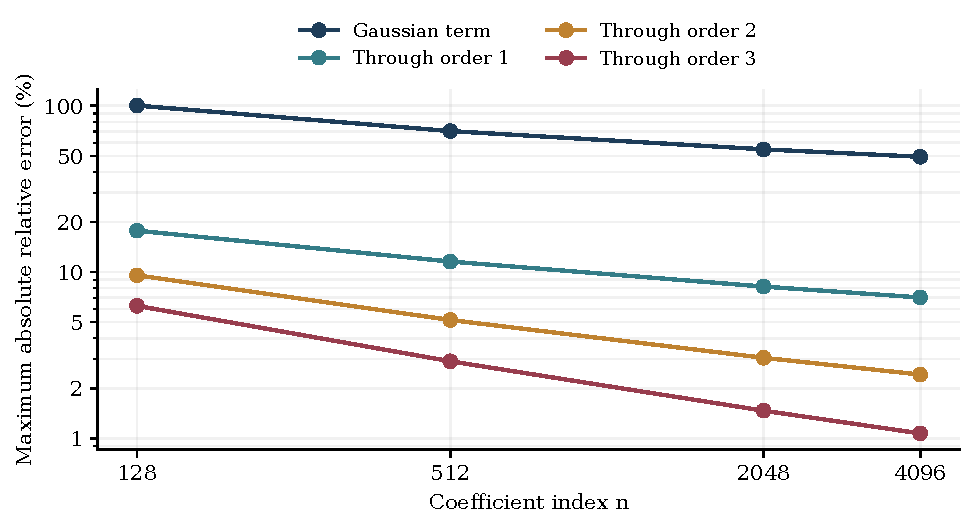
\includegraphics[width=0.91\textwidth]{figures/coefficient_refinement.pdf}
\caption{The errors in Table~\ref{tab:errors}, computed from finite
positive recurrences. The lines connect the four evaluated values of
$n$ and do not represent fitted convergence rates.}
\label{fig:refinement}
\end{figure}

The symbolic program verifies six total-degree identities through
degree five in the exponential--Stirling expansion; 36 central
Gamma-jet identities; and the five identities
$D_j=Q_j(-\log2)$ for $0\le j\le4$. The two algebraic routes use,
respectively, reciprocal Gamma products and positive-half-integer
Gamma moments. Nine noninteger-order Fourier quadratures, at 80
digits, check the parabolic cylinder normalization with absolute
errors below $10^{-65}$. Separate Fourier checks cover the order
derivatives used in the coefficient diagnostics. These computations
are sensitive to the Fourier sign and to the imaginary part of
$\Log(-iy)$.

For the inverse endpoint results, nine high-precision inverse
calculations cover $m=2,3,4$ and three small deficits $y$; six
upper-bank evaluations cover $s=1.25,1.4$ and three small $u$.
They agree with the proved reciprocal expansions and the negative
cut-modulus increment. The exact classifications in
Theorem~\ref{thm:ramification} follow from analytic continuation and
the displayed expansions, not from those samples.

Figure~\ref{fig:transition} illustrates only the normalized two-term
expression in Theorem~\ref{thm:wing-lambert}. This distinction matters:
the figure is an illustration of the explicit analytic profile,
whereas Figure~\ref{fig:refinement} compares independently computed
coefficients with their approximations.

\begin{figure}[htbp]
\centering
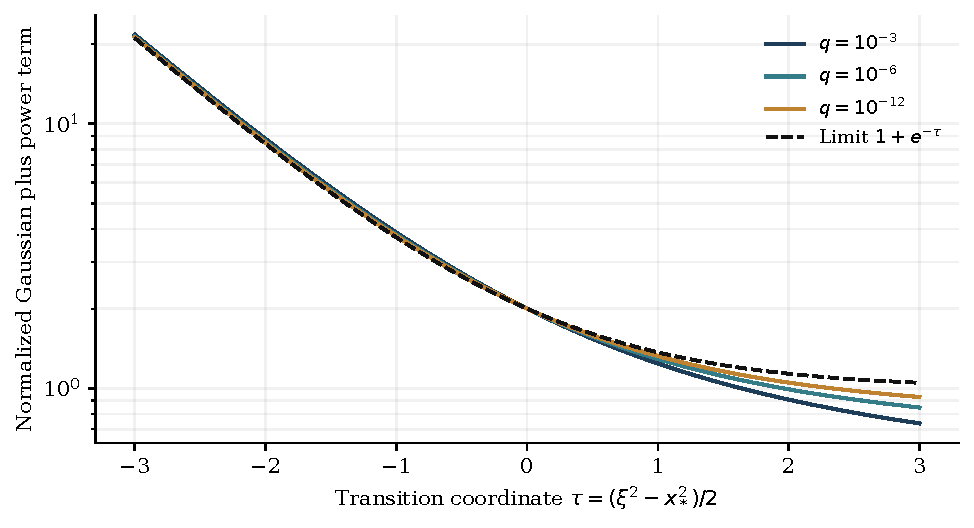
\includegraphics[width=0.91\textwidth]{figures/lambert_transition.pdf}
\caption{For $\xi=\sqrt{x_*(q)^2+2\tau}$, the exact normalized
two-term expression is
$e^{-\tau}+(1+2\tau/x_*(q)^2)^{-3/2}$.
The curves show this expression for three values of $q$ and its
limit $1+e^{-\tau}$. They are not sampled probabilities.}
\label{fig:transition}
\end{figure}
\FloatBarrier

\subsection{A focused audit and concrete proposed amendments}

No false printed theorem was established in the coefficient sources
used here. The useful corrections are statements of scope and
updates to explicit research questions. The accompanying
\mbox{\texttt{INTEGRATION.md}} gives proposed insertions without changing the
pinned repository. \path{THEOREM_LEDGER.md} records the hypotheses
and dependencies of each principal result. Source paths and hashes
are supplied in \path{PROVENANCE.json}.

\begin{enumerate}[label=\textbf{A\arabic*.},leftmargin=*]
\item \textbf{Mark the compact joint window of Q1 as resolved.}
Theorem~\ref{thm:all-orders} proves the requested joint coefficient
law, all fixed logarithmic corrections, and the uniform Fourier
bound. Equation~\eqref{eq:elementary-first} supplies the first
correction in the elementary scale requested there.
Equations~\eqref{eq:Lambert-scale}--\eqref{eq:matching} give the
exact marginal comparison. This is stronger than substituting
$s=s_n$ into a theorem whose constants were controlled only at
fixed $s$.

\item \textbf{Record a partial positive answer to Q2.}
Theorems~\ref{thm:positive-windows} and \ref{thm:wing-lambert}
give a relative approximation on every fixed polynomial window
in $\log n$, and an explicit transition profile. The negative
growing window and the passage to genuinely macroscopic
deviations remain open in this treatment.

\item \textbf{Retain the distinction between an endpoint value and
the coefficient radius.} The identity
$R_b^n a_n=\Prob(X_n=n)/n$ holds for every $b>0$.
The reference $R_b=e^{-(u-b)}$ is the actual radius on the
endpoint-controlled side $b\ge A$. For $b<A$, the principal
inverse encounters an interior fold and the radius is larger.
The uniform lattice estimate uses the reference value without
relabeling it as the radius below criticality.

\item \textbf{Add the reciprocal-order exception to endpoint
discussions.} The inverse endpoint is holomorphic at
$s=1+1/m$, $m\ge2$. An argument which treats every noninteger
polylogarithm branch point as a nonremovable inverse branch
point misses these exceptions. Theorem~\ref{thm:ramification}
gives the complete local replacement, with the minimal
ramification index. It makes no claim about other inverse
singularities at the same modulus.

\item \textbf{Qualify the proposed real-order extension of Q9.}
The cut-modulus inequality used for integer orders fails for
every $1<s<3/2$. Thus that proof cannot establish a blanket
real-order extension of the endpoint-circle statement in
\cite{repo-inverse}. This is a counterexample to the proposed
extension of the inequality, not to the existing integer theorem,
and it does not itself settle the global inverse Taylor radius.

\item \textbf{Keep the two convergence assertions separate.}
The implicit scale chart and the reciprocal-order inverse chart
are convergent holomorphic expansions. The coefficient series
is proved to every \emph{fixed} logarithmic order, with constants
depending on that order. Neither a convergent infinite Fourier
core expansion nor an optimal-truncation theorem is proved.
Uniform absolute error over all lattice points is also distinct
from a relative approximation where the probability vanishes.
The positive-window proof supplies the additional estimate in
exactly the range where it is used.
\end{enumerate}

\subsection{Further research questions with concrete starting points}

The following questions separate direct extensions from problems
requiring a different analytic mechanism. None is needed for the
validity of the results above.

\begin{enumerate}[label=\textbf{R\arabic*.},leftmargin=*]
\item \textbf{What is the relative law on growing negative
windows?} The Fourier theorem supplies an absolute error there,
but the algebraic positive tail is absent. A saddle displacement
on the negative side should be combined with the pole-paired
exponent before truncation. A useful first target is a relative
theorem for $-L^M\le\xi\le-r_L$, identifying the largest $M$
for which a finite expansion in the same parameters suffices.
This would address the remaining side of Q2 and quantify the
onset of the interior-fold regime.

\item \textbf{Can one join the compact resonance window to the
stable and finite-variance regions at every correction order?}
Here $|\lambda|$ is bounded. Letting $\lambda$ tend to either
infinity in the displayed formulas is not justified by this
proof. The leading all-rate results in \cite{repo-confluent}
suggest an overlap problem: construct uniform normalizations
and remainders when $\lambda=\lambda_n$ grows, then match to
fixed-order stable or finite-variance expansions. The exact
function $K_\eps$ is a natural common coordinate, but the
Fourier truncation and error constants must be redesigned.

\item \textbf{What is the first sector beyond all logarithmic
orders, and how does it remember the nonlinearity?}
The composition theorem removes all endpoint derivatives of
$G$ beyond the second from the fixed logarithmic sector.
Retain the cubic terms in
$G(\zeta(s)-D_s(t))$ and scale them by $nB^{-3}$.
This gives a concrete route to the first smaller sector,
including the first dependence on $G'''(\zeta(s))$.
The question is to prove a uniform mixed expansion in powers
of $B^{-1}$ and inverse logarithms, with a transparent
description of which endpoint derivatives first occur in
each sector.

\item \textbf{How fast do the coefficient functions grow with
the truncation order?} The finite formulas reduce this to
joint large-order estimates for Stirling numbers and
$\HH_{2k}^{[j]}$. Determine a useful Gevrey bound on compact
spatial sets, investigate optimal truncation, and identify the
associated exponentially small remainder. Any summation
procedure must respect the Fourier tail: the untruncated
exponential obtained from the local model need not be
integrable on the full real line. Formal exponentiation
alone therefore cannot supply this result.

\item \textbf{How far can the relative positive window be
extended?} The present argument reaches $\xi\le L^M$ for
every fixed $M$, by choosing a sufficiently large but fixed
logarithmic order. For displacements of algebraic size in
$n$, this argument loses relative control. A direct uniform
local large-deviation estimate for the triangular compound
Poisson family could bridge the gap to fixed supercritical
$b>A$, while keeping the exact amplitude
$b^{s-1}(b-A)^{-s}$. The work of \cite{berger} is an
appropriate starting point for the required probability
estimates, with the moving-law uniformity proved explicitly.

\item \textbf{What determines the global inverse radius at a
removable reciprocal endpoint?} Local removal of the value
$\zeta(1+1/m)$ does not locate the next singularity of the
inverse germ. Determine which critical values, asymptotic
values, or sheet obstructions first meet its continuation.
Potential critical points away from zero satisfy
$\Li_{1/m}(z)=0$. Even the case $m=2$ would clarify whether
other singularities can retain the endpoint modulus after
the positive endpoint itself becomes removable.

\item \textbf{Can order jets and ramification be organized
uniformly in the jet index?} The convergent reciprocal chart
handles every fixed jet and compact $\tau$.
The leading term shows that differentiation in order restores
logarithms despite local removability at the central order.
Determine the allowable joint growth of the derivative
index, $|\log y|$, and the winding number. This would connect
the exact monodromy and order-jet calculus of the existing
Polylogarithms chapters with quantitative inverse estimates.

\item \textbf{What is the sharp positivity hypothesis for
composition universality?} The sufficient condition
$G'(0)>0$ gives a uniform coefficient lower bound and
aperiodicity immediately. Some positive outer functions
with $G'(0)=0$ may still have the needed tail mass and
lattice span after composition. Characterize the weakest
conditions that yield the two Fourier bounds, and then
separate these probabilistic conditions from the local
analytic conditions at $\zeta(s)$.

\item \textbf{Can several colliding tail terms be treated by
one finite calculus?} Replace a single polylogarithm by a
positive combination with orders moving through the same
integer, or add controlled slowly varying factors obtained
by order differentiation. The scalar divided difference
suggests a multivariate Stirling or Bell-polynomial
description. The challenge is to choose a normalization
that preserves uniform positivity and keeps all pole
cancellations explicit.

\item \textbf{Which part should be formalized first?}
A tractable initial layer consists of the finite
coefficient--probability identity, the Gamma recurrence
pairing, the Stirling coefficient formula, and the
reciprocal-order Lagrange identities. The analytic layer
then needs parameter-uniform Fourier inversion,
dominated convergence with logarithmic powers, and
holomorphic implicit inversion. This separation would
produce reusable formal components rather than a
single opaque formalization of the final theorem.
\end{enumerate}

The central structural point is that the collision at $s=3$ can be
absorbed into an exact scale while leaving a finite order-derivative
calculus for every correction. Positivity provides the global Fourier
control needed to turn that local calculus into a theorem. The
reciprocal inverse endpoints exhibit the complementary phenomenon:
ramification can disappear at an exceptional order, while its
logarithmic dependence remains visible to differentiation in order.
